\subsection{Ablation Study}


\begin{figure}[ht!]
    \centering
    \begin{subfigure}[b]{0.45\linewidth}
        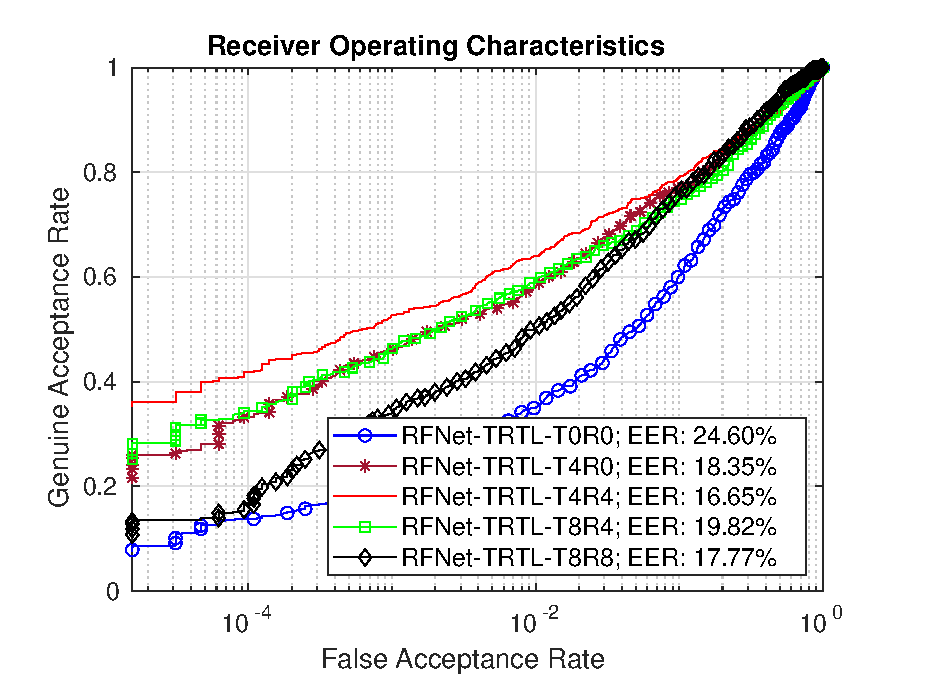
\includegraphics[width=\linewidth]{Figures/ablation-roc_compare_new.eps}
        \caption{}
    \end{subfigure}
    \begin{subfigure}[b]{0.45\linewidth}
        \includegraphics[width=\linewidth]{Figures/ablation-cmc_compare_new.eps}
        \caption{}
    \end{subfigure}
    \caption{Comparative ROC (a) and corresponding CMC (b) for two-session of the Finger Knuckle Database (Version 3.0) \cite{fingerknuckledbv3.0}. For approving our TRTL loss function efficiency, we change the translation parameter and rotation parameter to show the different matching performance.}
    \label{ablation-study}
\end{figure}

\begin{figure}[ht!]
    \centering
    \begin{subfigure}[b]{0.45\linewidth}
        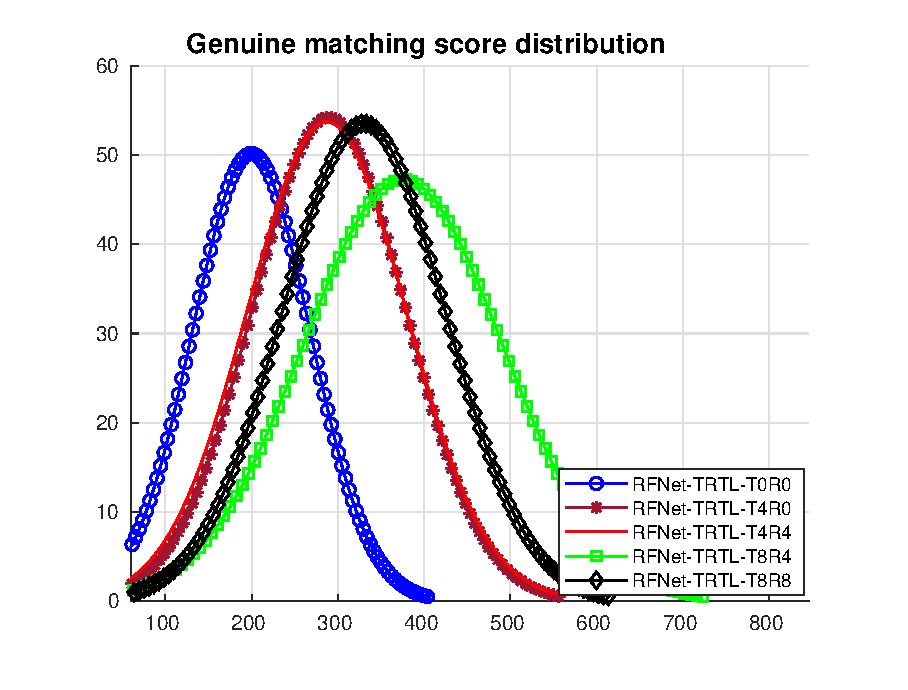
\includegraphics[width=\linewidth]{Figures/ablation-genuine_distribution.eps}
        \caption{}
    \end{subfigure}
    \begin{subfigure}[b]{0.45\linewidth}
        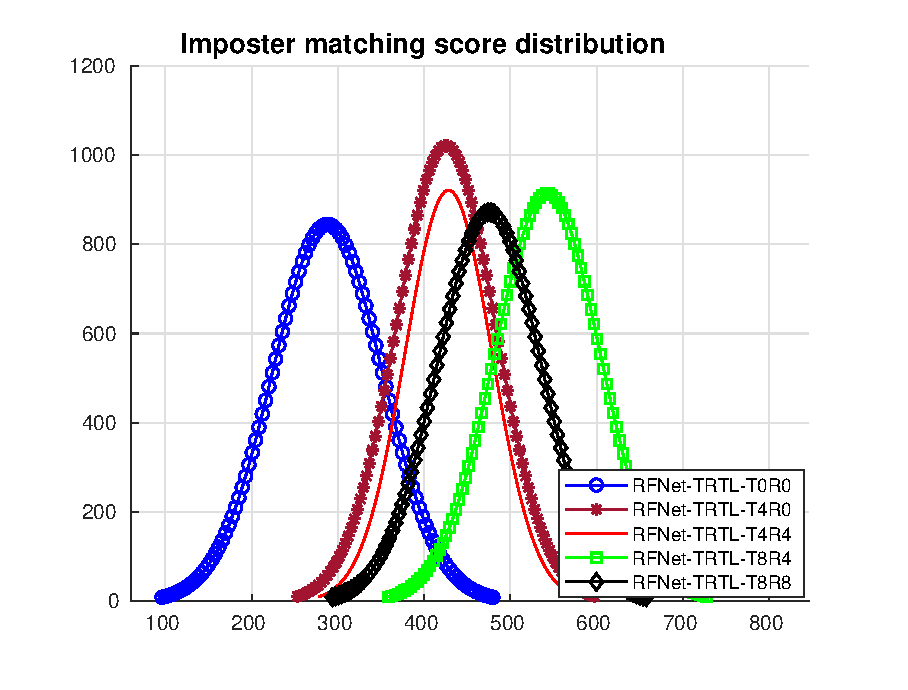
\includegraphics[width=\linewidth]{Figures/ablation-imposter_distribution.eps}
        \caption{}
    \end{subfigure}
    \caption{Genuine matching score distribution (a) and Imposter matching score (b) for two-session of the Finger Knuckle Database (Version 3.0) \cite{fingerknuckledbv3.0}. For approving our TRTL loss function efficiency, we change the translation parameter and rotation parameter to show the different matching performance.}
    \label{ablation-study-distribution}
\end{figure}

.........